%% LyX 2.3.1-1 created this file.  For more info, see http://www.lyx.org/.
%% Do not edit unless you really know what you are doing.
\documentclass[turkish]{eqconf}
\usepackage[T1]{fontenc}
\usepackage[utf8]{inputenc}
\usepackage{wrapfig}
\usepackage{amsmath}
\usepackage{accents}
\usepackage{graphicx}
\usepackage{blindtext}
%\usepackage{showframe}

\makeatletter

%%%%%%%%%%%%%%%%%%%%%%%%%%%%%% LyX specific LaTeX commands.
\newcommand{\docedilla}[2]{\underaccent{#1\mathchar'30}{#2}}
\newcommand{\cedilla}[1]{\mathpalette\docedilla{#1}}

%% Because html converters don't know tabularnewline
\providecommand{\tabularnewline}{\\}


%%% Optional Math Operation: Makes bold greek letters more bold
\usepackage{upgreek}%Needed for Matrix Greek Letters
\usepackage{pdfrender}%Needed for Matrix Greek Letters
\newcommand*{\boldgreek}[1]{%
	\textpdfrender{%
		TextRenderingMode=FillStroke,%
		LineWidth=.35pt,%
	}{#1}%
}

\title{BİLDİRİ BAŞLIĞI BİLDİRİ BAŞLIĞI BİLDİRİ BAŞLIĞI\\
	BİLDİRİ BAŞLIĞI BİLDİRİ BAŞLIĞI BİLDİRİ BAŞLIĞI}
\author{\authorname{1}{Ahmet Yılmaz},
		\authorname{1}{Mustafa Mehmet Kaya} ve
		\authorname{2}{John Doe}}

\date{\affils{1}{Araş. Gör., İnşaat Müh. Bölümü, Abece Üniversitesi, Güzelkent}\\
	\affils{2}{Prof. Dr., Jeofizik Müh. Bölümü, Abece Teknik Üniversitesi, Büyükkent}\\
	\email{gönderenyazar@kurum.edu.tr}%%% Sadece gönderen yazarın e-postası girilecektir.
}

%%Biblatex
\usepackage{etoolbox}
\AtEndPreamble{%
	\DefineBibliographyStrings{english}{%
		references = {{KAYNAKLAR}},
		and = {ve},
		andothers = {vd.},
		pages = {s.},}
		\renewbibmacro{in:}{}
		\usepackage{csquotes}
}
	
\makeatother

\usepackage{babel}
\usepackage{xkeyval}

\usepackage[style=authoryear,maxcitenames=2,
doi=false,isbn=false,url=false,
eprint=false,giveninits]{biblatex}
\addbibresource{examplebib.bib}



\begin{document}
%%%%%% Keep thes lines %%%%%
\fixturkishbug %% For the Turkish-\includegraphics bug
\maketitle \thispagestyle{firststyle} %%%%%%%

%%% A Turkish Abstract has to be provided if the paper is in Turkish
\begin{ozet} \blindtext \end{ozet}

\begin{anahtarkelimeler} anahtar kelime1, anahtar kelime2, anahtar
kelime3. \end{anahtarkelimeler}

%%% All papers (both Turkish and English) have to provide English abstract

\begin{abstract}
\blindtext 
\end{abstract}
\begin{keywords} keyword1, keyword2, keyword3. \end{keywords}

\section{GİRİŞ BÖLÜMÜ}

\blindtext 
\begin{equation}
%Denklemden\ddot{o}ncebo\cedilla{s}lukb\imath rak\imath lmamal\imath
x=\dfrac{a}{b},\quad\boldgreek{\alpha}=\boldgreek{\upphi}\label{eq:massdef}
\end{equation}

\blindtext

Görüldüğü üzere, sonuçların doğru olduğu anlaşılmaktadır. Hatalı sonuçlar
için başka yorumların yapılması uygun olacaktır (\cite{Skinner1993}).

\section{TEORİ BÖLÜMÜ}

\blindtext

\subsection{Denklemler}

\blindtext 
\begin{equation}
%Denklemden\ddot{o}ncebo\cedilla{s}lukb\imath rak\imath lmamal\imath
g(x)=\int_{a}^{b}f(x)dx,\quad x=\dfrac{a}{b},\quad\boldgreek{\alpha}=\boldgreek{\upphi}\label{eq:energy}
\end{equation}

Denklem (\ref{eq:energy})'de de görüldüğü üzere, sonuçların doğru
olduğu anlaşılmaktadır. Hatalı sonuçlar için başka yorumların yapılması
uygun olacaktır. \textcite{Narasimhan2006,Erkus2006}'de gösterildiği
üzere, yapılan çalışmaların uygun olduğu anlaşılmaktadır.

\blindtext

\subsection{Diğer Bilgiler}

\blindtext

Şekil (\ref{fig:structure})'de de görüldüğü üzere, sonuçların doğru
olduğu anlaşılmaktadır. Hatalı sonuçlar için başka yorumların yapılması
uygun olacaktır.

\blindtext

\begin{wrapfigure}{r}{0.4\textwidth}%
 \vspace{-12pt}
 \centering 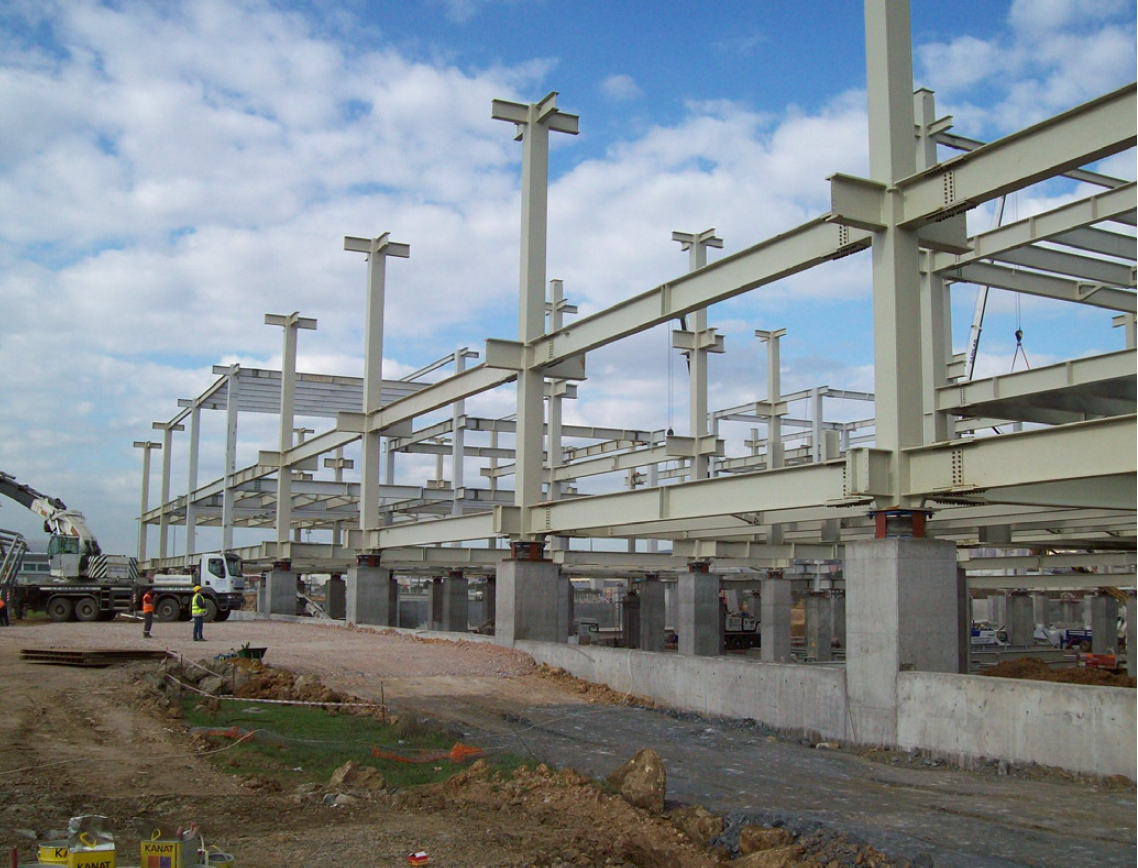
\includegraphics[scale=0.2]{b.PNG} \caption{\label{fig:structure}Bir bina yapısı.}
\vspace{-10pt}
 \end{wrapfigure}%

\blindtext

Şekil (\ref{fig:otherstruct})'de de görüldüğü üzere, sonuçların doğru
olduğu anlaşılmaktadır. Hatalı sonuçlar için başka yorumların yapılması
uygun olacaktır.

\begin{figure}
\centering 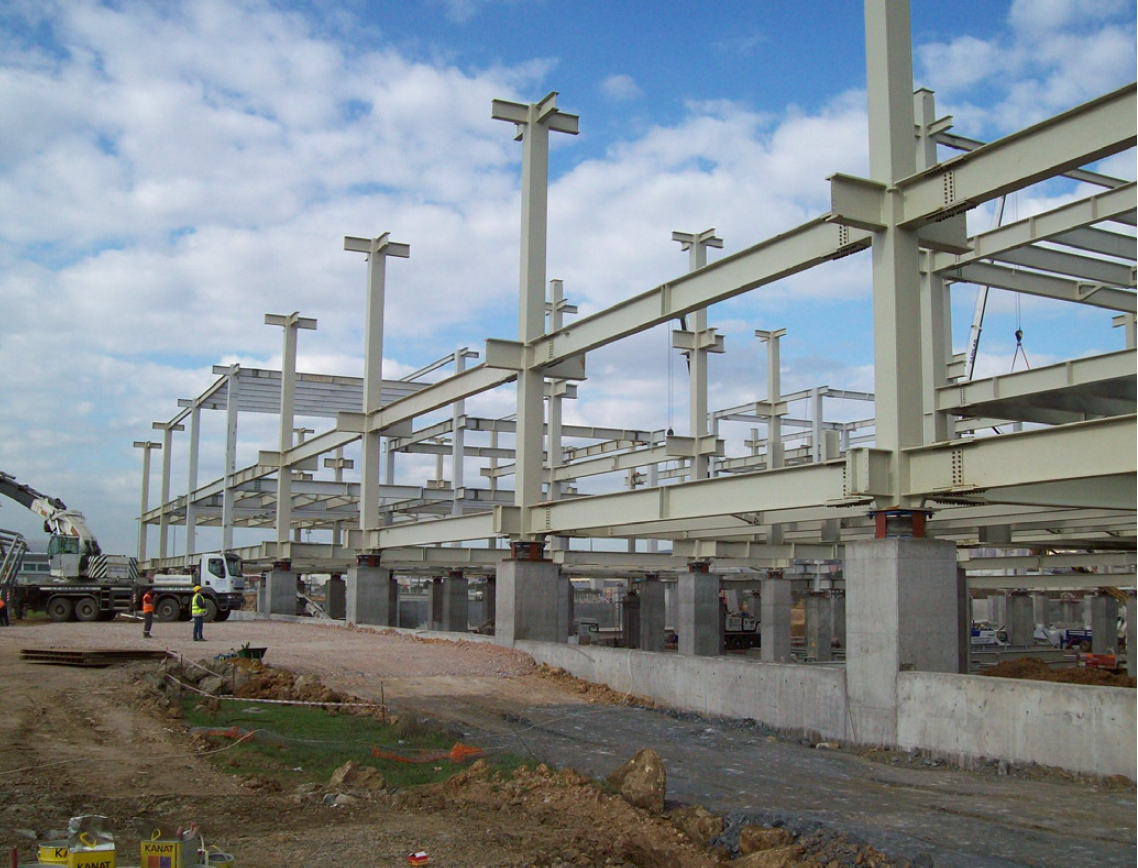
\includegraphics[scale=0.4]{b.PNG} \caption{\label{fig:otherstruct}Diğer bina.}
\end{figure}
\blindtext 
\begin{equation}
%Denklemden\ddot{o}ncebo\cedilla{s}lukb\imath rak\imath lmamal\imath
g(x)=\int_{a}^{b}f(x)dx,\quad x=\dfrac{a}{b},\quad\boldgreek{\alpha}=\boldgreek{\upphi}\label{eq:stiffness}
\end{equation}

Denklem (\ref{eq:stiffness})'de de görüldüğü üzere, sonuçların doğru
olduğu anlaşılmaktadır. Hatalı sonuçlar için başka yorumların yapılması
uygun olacaktır.

\blindtext

\subsubsection*{Alt Alt Başlık}

\blindtext

\blindtext

\subsection{Başka Diğer Bilgiler}

\blindtext

\blindtext

%	\vspace{-5pt}
\begin{table}
\setlength{\abovecaptionskip}{-5pt} \setlength{\belowcaptionskip}{10pt}
\centering \caption{\label{tab:onemlibilgi}Önemli Bilgiler.}
\begin{tabular}{l|c|r}
% <-- Alignments: 1st column left, 2nd middle and 3rd right, with vertical lines in between
\textbf{Value 1}  & \textbf{Value 2}  & \textbf{Value 3}\tabularnewline
$\alpha$  & $\beta$  & $\gamma$ \tabularnewline
\hline 
1  & 1110.1  & a\tabularnewline
2  & 10.1  & b\tabularnewline
3  & 23.113231  & c\tabularnewline
\end{tabular}
\end{table}
Tablo (\ref{tab:onemlibilgi})'de de görüldüğü üzere, sonuçların doğru
olduğu anlaşılmaktadır. Hatalı sonuçlar için başka yorumların yapılması
uygun olacaktır.

\blindtext

\blindtext

\section{YENİ BÖLÜM}

\blindtext

\blindtext

\subsection{Başka Diğer Bilgiler}

\blindtext

\subsection{Başka Başka Diğer Bilgiler}

\blindtext

\begin{wraptable}{l}{6cm}%
 \setlength{\abovecaptionskip}{0pt} \setlength{\belowcaptionskip}{15pt}
\vspace{-10pt}
 \centering \caption{\label{tab:baskasonuc}Başka sonuçlar.}
\begin{tabular}{l|c|r}
% <-- Alignments: 1st column left, 2nd middle and 3rd right, with vertical lines in between
\textbf{Value 1}  & \textbf{Value 2}  & \textbf{Value 3}\tabularnewline
$\alpha$  & $\beta$  & $\gamma$ \tabularnewline
\hline 
1  & 1110.1  & a\tabularnewline
2  & 10.1  & b\tabularnewline
3  & 23.113231  & c\tabularnewline
\end{tabular}\vspace{-10pt}
 \end{wraptable}%

Tablo (\ref{tab:baskasonuc})'de de görüldüğü üzere, sonuçların doğru
olduğu anlaşılmaktadır. Hatalı sonuçlar için başka yorumların yapılması
uygun olacaktır.

\blindtext

\subsubsection*{Alt Alt Başlık}

\blindtext

\blindtext

\subsection{Başka Diğer Bilgiler}

\blindtext

\blindtext

\begin{figure}[h]
\centering 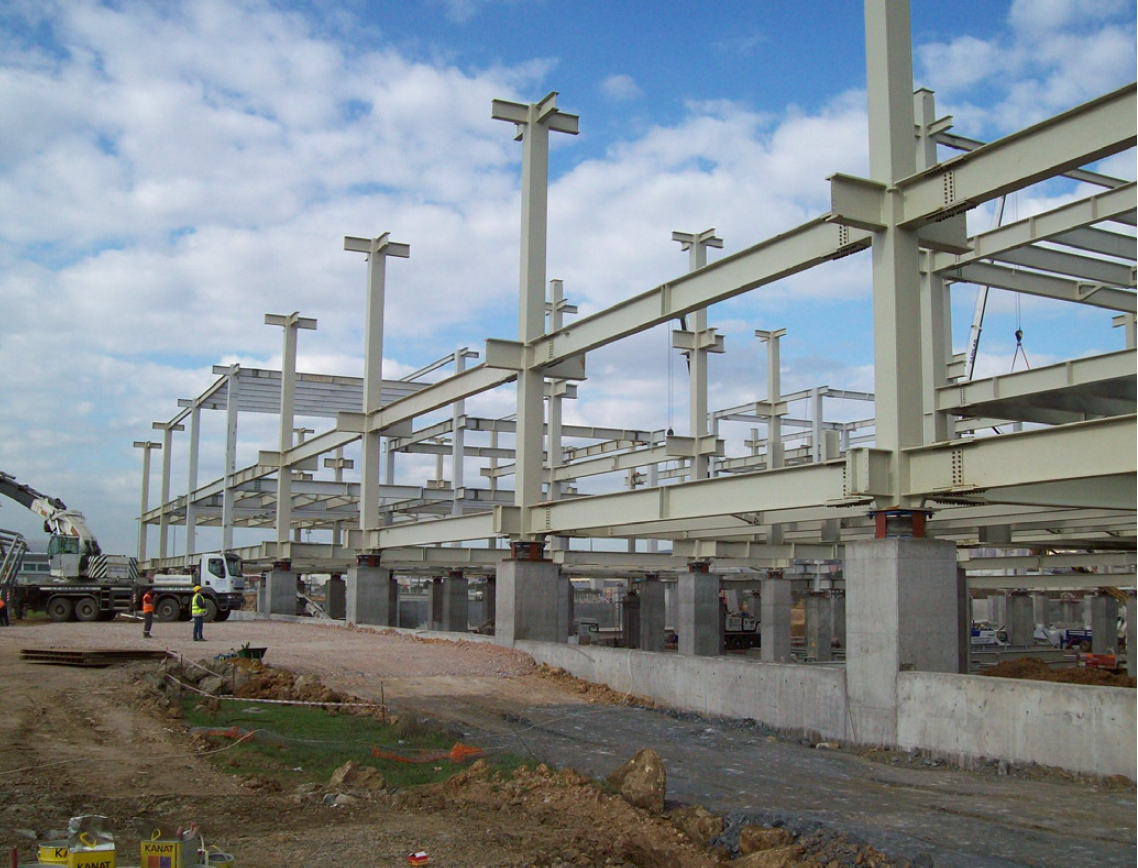
\includegraphics[scale=0.4]{b.PNG} \caption{\label{fig:ikinciyapi} Başka başka şekiller.}
\end{figure}
Şekil (\ref{fig:ikinciyapi})'de de görüldüğü üzere, sonuçların doğru
olduğu anlaşılmaktadır. Hatalı sonuçlar için başka yorumların yapılması
uygun olacaktır.

\blindtext

\section{SONUÇ}

\blindtext

\blindtext

\printbibliography

\end{document}
